\chapter{開発プロセス}

\section{前期第1プロセス}

\subsection{ヒアリング}
我々は町会の置かれている現状を明らかにするため,
5月12日に町会の会長, 副会長, 総務部長, 会計部長, 青少年育成部副部長に対して,
我々は学部3年生5名とTA5名と教員4名でヒアリングを行った.
町会役員から\ref{problems}で述べたイベント開催に関する問題と以下の要望が明らかになった.

\begin{itemize}
\item 開催予定のイベント一覧をカレンダーで表示して欲しい.
\item iOSのアプリケーションを作って欲しい.
\item 幅広い年代の人が使いやすいUIにして欲しい.
\item 町会の役員の数を増やすため, 町内会を知ってもらいたい.
\item イベント発信をした際に通知できる機能が欲しい.
\item イベントスケジュールでイベントの削除, 作成, 更新ができるようにして欲しい.
\item 行事をタップしたらそのまま参加申し込みフォームに遷移して欲しい.
\item 保護者の方の確認を得るためのポップアップ機能が欲しい.
\item イベントで不参加になった人が分かるようにして欲しい.
\end{itemize}

我々は, これらの要望を取り入れつつ問題を解決するアプリケーションを開発することとした.
\bunseki{永井陽太}


\subsection{アプリケーションアイデアの考案}
\ref{problems}で述べた問題と町会の要望を分析した結果, イベントに関する内容のものが多かった.
そこでイベントに関係する3つの問題を解決することとした. 問題は
「FacebookやLINE@ではイベントに関するお知らせはできるが, 開催予定のイベントを一覧で見れない」
「Facebookでは個人情報が漏れてしまうため参加申し込みができない」
「役員だけで共有したい情報を町民に知られずに共有することがFacebookやLINE@ではできない」の3つである.
これらの問題を解決するために, 開催予定イベントのカレンダー表示機能,
イベントへの参加申し込み機能, 参加申し込み者の情報を役員のみが見ることのできる機能,
役員のみが役員会議などのイベント情報を見ることのできる機能を考案した.
アプリケーションアイデアの一部であるイベントカレンダー画面(図\ref{calender}),
参加フォーム画面(図\ref{joinform}), イベント作成画面(図\ref{create_event.old})を以下に示す.

\newpage
\begin{figure}[h]
    \begin{tabular}{ccc}
      %---- 最初の図 ---------------------------
      \begin{minipage}[t]{0.33\hsize}
        \centering
        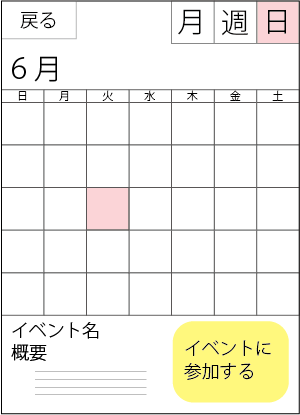
\includegraphics[keepaspectratio, scale=0.4]{process_figures/calender.png}
        \caption{イベントカレンダー画面}
        \label{calender}
      \end{minipage} &
      %---- 2番目の図 --------------------------
      \begin{minipage}[t]{0.33\hsize}
        \centering
        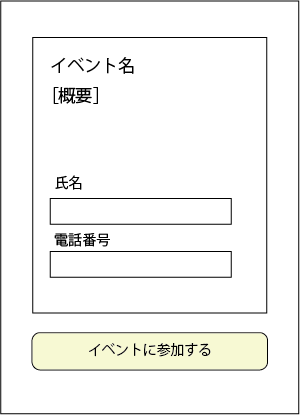
\includegraphics[keepaspectratio, scale=0.4]{process_figures/joinform.png}
        \caption{参加フォーム画面}
        \label{joinform}
      \end{minipage}
      %---- 3番目の図 --------------------------
      \begin{minipage}[t]{0.33\hsize}
        \centering
        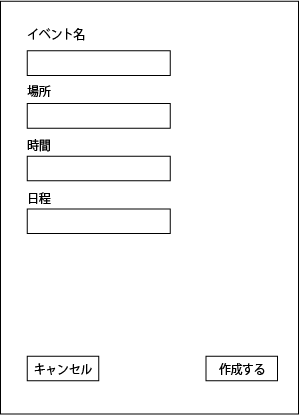
\includegraphics[keepaspectratio, scale=0.4]{process_figures/old_create_event.png}
        \caption{イベント作成画面}
        \label{create_event.old}
      \end{minipage}
      %---- 図はここまで ----------------------
    \end{tabular}
\end{figure}
\bunseki{永井陽太}

\subsection{第1回提案}
\label{first_review}
5月30日に我々が考えたアプリケーションの画面イメージを町会に提案した.
その結果, iOS, Android, Webアプリケーションの3つに対応可能なアプリケーション開発を行うことが決定した.
また, 我々の考案したアプリケーションイメージについて, レビューで3つの要望を得た.
1つ目は, イベント参加者の名簿を市役所に提出する際に参加者の情報として「名前」「性別」「年齢」「住所」「電話番号」が必要なので,
図\ref{joinform}の入力フォームに5つの情報を追加して欲しいという要望である.
2つ目は, アプリケーションをインストールした人が, すぐイベントを確認できるように起動時の画面はログイン画面にしないで欲しいという要望である.
3つ目は, 図\ref{create_event.old}に「定員」の項目を追加して欲しいという要望である.
\bunseki{永井陽太}

\section{前期第2スプリント}

\subsection{第1回月例レビュー会}
月例レビュー会とは, プロジェクト内で, 3つのチームが現在の進捗報告と今後の展望を発表し, その発表内容に対して担当教員, TA, 他チームのメンバーからレビューを受ける会である.
ここで我々は, 現在のアプリケーションアイデア, つまり, 役員と町民でイベントカレンダーを共有する機能で本当に問題を解決できているのかと教員より指摘を受け,
\ref{first review}にうけたレビュー内容も考慮し, アプリケーションについて再考し改善を図った.


\subsection{アプリケーションアイデアの改善}
改善の結果, カレンダーを用いて開催予定のイベントを表示するのではなく,
開催予定のイベントを直近のものから順にリスト表示することにした.
なぜなら, カレンダー表示では来月の予定などがひと目で確認することができないからである.
アプリケーションアイデアの一部であるイベントリスト画面(図\ref{eventlist}),
イベント作成画面(図\ref{new_create_event}), 参加者リスト画面(図\ref{joinedlist})を以下に示す.

%\newpage%苦肉の策
\begin{figure}[h]
    \begin{tabular}{ccc}
      %---- 最初の図 ---------------------------
      \begin{minipage}[t]{0.3\hsize}
        \centering
        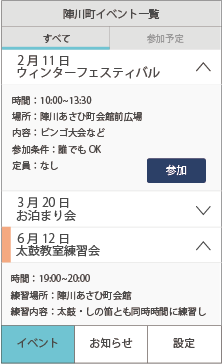
\includegraphics[keepaspectratio, scale=0.5]{process_figures/eventlist.png}
        \caption{イベントリスト画面}
        \label{eventlist}
      \end{minipage} &
      %---- 2番目の図 --------------------------
      \begin{minipage}[t]{0.3\hsize}
        \centering
        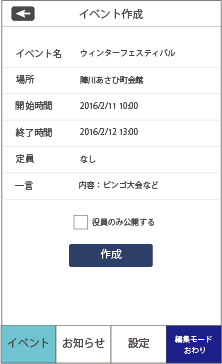
\includegraphics[keepaspectratio, scale=0.5]{process_figures/new_create_event.png}
        \caption{イベント作成画面}
        \label{new_create_event}
      \end{minipage}
      %---- 3番目の図 --------------------------
      \begin{minipage}[t]{0.3\hsize}
        \centering
        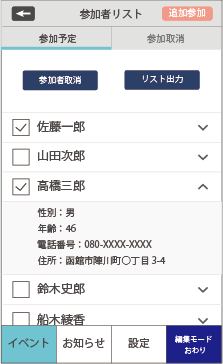
\includegraphics[keepaspectratio, scale=0.5]{process_figures/joinlist.png}
        \caption{参加者リスト画面}
        \label{joinedlist}
      \end{minipage}
      %---- 図はここまで ----------------------
    \end{tabular}
\end{figure}
\bunseki{永井陽太}

\subsection{第2回提案}
6月23日に我々は町会に対して改善したアプリケーションイメージを提案した.
その結果, 画面ごとにレビューしてもらい詳細な要望を受けた.
具体的には, 図\ref{eventlist}でイベントをタップすると画面いっぱいにイベントの詳細情報が表示されるようにして欲しいという要望,
図\ref{new_create_event}にアプリケーションの所有者全員に通知するか, しないかの項目を設けて欲しいという要望である.
また, 町民が利用したくなるようなコンテンツを追加して欲しいという要望も得た.
過去のイベントの写真が確認できるWebページとアプリケーションとリンクさせることが例として挙げられる.
\bunseki{永井陽太}

\section{前期第3スプリント}

\subsection{中間発表}
%----中間発表の内容-----------------
7月8日に行われた中間発表では, 各グループが行ってきた活動を詳細に伝え, 後期の活動に活かせるレビューをもらうことを目的とした.
そのため全体ポスター2分, 各グループのポスターとデモを含めた発表を12分間並行して発表を行った.
\bunseki{伊藤泰斗}

\subsubsection{発表方法についての評価と振り返り}
以下に, 中間発表会で行ったアンケートの「発表技術について」の項目から, メンバ間で精査した結果, 最終成果発表にも取り入れたいコメントを抜粋した.
\begin{itemize}
  \item デモがプロトタイプであることを伝えないと, 実装したものだと勘違いしてしまう.
  \item もう少しスラスラ話せていたら分かりやすかったと感じた.
\end{itemize}
    上記より, 伝える情報とポスターセッションの練習の不足が伺える.
    しかし, 「とても喋りに安定感があるなと感じた」との評価も受けた. 最終成果発表の際にはすべて開発したアプリケーションでデモを行い,
    ポスターセッションをする人全員がスラスラと話せるくらいに練習を行っていく.

\subsubsection{発表内容についての評価と反省}
    「発表内容について」の項目から後期の開発や発表において考慮すべきコメントを抜粋した.
\begin{itemize}
  \item 陣川町民に使ってもらうためのプロモーションの方法を考えたほうが良い
  \item クーポンなど, ユーザを得る工夫が欲しい
  \item ユーザにより沿って開発していく中で生起した出来事を大切に記述して欲しい
\end{itemize}
    上記より, 2つの見落としが伺えた. 1つ目はユーザに使ってもらうための考慮をしていなかったことである.
    メンバ全員が使ってもらえることを前提として考えていることである. しかし実際には使ってもらえることは前提ではないため,
    どのようにして使ってもらうのかを考える必要がある. 2つ目は, 本アプリケーションにユーザにとって魅力的な優位性が必要であることである.
    認知されていてもユーザにとって使いたいものでなければ使ってもらうことができない. そのため, 最終成果発表までにプロモーションの方法を考え,
    使ってもらうための工夫を本アプリケーションに追加することでユーザを獲得していきたい.
\bunseki{伊藤泰斗}


\subsection{第1回集中実装}
 夏季休業期間中に, じぷりの主要な機能の内の「イベントの編集・削除機能」, 「お知らせの削除機能」, 「イベントへの参加申し込み機能」を実装した.
%----集中開発の内容-----------------

\section{後期第1スプリント}
\subsection{後期活動開始}
\subsubsection{プロダクトバックログ・スプリントバックログの導入}
 前期のプロジェクト活動では、アジャイル開発手法の1つスクラム開発を行っていたものの、スプリントバックログや、プロダクトバックログの作成を行っていなかったので、
後期の活動からスプリントの始まりに、タスクを洗い出し、担当を割り振り、期日を設けてスプリントバックログとプロダクトバックログを作成することを決定した。todo/実際のバックログを載せる。

\subsubsection{チーム内のルール制定}
 後期の活動からは”チーム運用ルール”を制定して活動していくことになったので、メンバで話し合いを行い、ルールを制定した。実際に制定されたルールは、
\begin{enumerate}
    \item 必ず定時の18:00に5人での作業を中断する
    \item 専門用語を使うときは説明できようにする。また、使いすぎないようにする
    \item 最終報告書を作成のコストを削減するために、議事録の最後に活動のまとめを書く
    \item 2週間に1回、活動のKPTG分析を行う
    \item 議事録担当を横山、永井、森島、船木、伊藤の順で回す
    \item 活動冒頭10分は個人タスクの進捗報告を行う
    \item プロジェクト活動終了時間40分前に活動をやめて、10分間チーム内でまとめを行う
    \item 町会との連絡には「jinnovation会議」というLINEグループを利用する
\end{enumerate}
上記の様になっている。
このようなルールが制定された理由を以下に記述する。
\begin{enumerate}
    \item 前期の活動で、時間外活動がプロジェクト内の3チームで一番多かったので時間外活動を減らすためである。
    \item 前期の活動で、情報システムコースと情報デザインコースで学習してきた内容に差異があるので、専門用語を利用して、メンバを困惑させる場面が多々あったので、そのような場面を回避するためである。
    \item 前期の活動報告書作成にコストがかかってしまい、開発に時間をかけることができなったので、後期ではそのような事態を回避するため。
    \item メンバの1人が夏季休業中のインターンシップで振り返りの際にkptg分析を行っていたので、実際に企業が行っていることをプロジェクト活動にも取り入れることで活動を振り返り、次に繋げられると考えたため。
    \item 前期の活動で議事録の担当をリーダーが覚えている限り均等になるように割り振っていたので、個人の記憶に頼るのではなく、ルールに則ることで、より均等になるように割り振るため。
    \item 前期の活動で、誰がどのタスクをどこまで終わらせていて、どこに困っているのかを共有する時間が、プロジェクト活動時間外に行われていたので、メンバ同士のリアクションも遅れてしまい、進捗を遅らせてしまっていたので、
          プロジェクト活動時間内に進捗報告を行うことで、メンバが困っていることを共有し迅速に解決することが出来るようにするため。
    \item プロジェクト活動最後の20分間にプロジェクト内で各チームの進捗と次回の活動内容とそれまでの個人のタスクの報告を行っていたのだが、前期の活動ではまとめの時間を明確に設けていなかったので、
          最後の20分間の報告の際に、次回やることや次回までのタスクを明確にして報告することができなかったので、そのような事態を回避するため。
    \item 前期の活動で、先方との連絡はリーダーを通して行われていたのだが、リーダーから先方との連絡の内容がメンバに十分に共有されておらず、
          明確にしなければならない疑問点などが町会との打ち合わせの直前にメンバから挙げられて慌てて先方に確認するという場面が多々あったので、そのような事態を回避するため。
\end{enumerate}




\section{後期第2スプリント}
\subsection{じぷりデザインの改善}
\subsection{町会打ち合わせ}
\subsection{第2回月例レビュー会}

\section{後期第3スプリント}
\subsection{アカデミックリンク}
\subsection{町会打ち合わせ}

\section{後期第4スプリント}
\subsection{町会打ち合わせ}
\subsection{最終成果発表}
